\documentclass[a4paper, 12pt]{report}
\usepackage{hyperref}
\usepackage{gensymb}
\usepackage{ amssymb }
\usepackage[utf8]{inputenc} % выбор кодировки кода
\usepackage[T2A]{fontenc} % выбор внутренней кодировки 
\usepackage[english, russian]{babel} % выбор языка
\usepackage{csquotes}
% \righthyphenmin = 2 % минимальное число букв после переноса: может пригодиться
\usepackage{multirow}
\usepackage{fontawesome}
\usepackage{easyReview}
\usepackage{tabularx}
\usepackage{rotating}
\usepackage{amsmath} % русский текст в формулах
\usepackage{color} % цвет текста
\usepackage{ulem} % для зачёркивания текстаё

\usepackage[left=15mm, right=10mm, top=20mm, bottom=20mm]{geometry} % поля
\usepackage{indentfirst} % отступ первого абзаца
\setlength{\parindent}{1,25cm} % длина отступа первой строки абзаца
\linespread{1,5} % междустрочный интервал

\usepackage{titlesec} % настройка заголовков
\renewcommand{\thesection}{\arabic{section}} % противотараканная мера для report'а: делаю section заголовком первого уровня
\titleformat{\section}{\centering \large \bfseries}{\thesection}{1ex}{\MakeUppercase}{}
\titleformat{\subsection}{\centering \large \bfseries}{\thesubsection}{1ex}{}{}
\titleformat{\subparagraph}[runin]{\bfseries}{\thesubparagraph}{}{}{}

% \titleformat{\bibliography}{\centering \large \bfseries}{\thebibliography}{}{}{} % попытка настроить заголовок для списка литературы

\usepackage{graphicx}
\usepackage{wasysym}

\usepackage{comment} % Для многострочных комментариев
\usepackage{xcolor} % Для девочек 
\usepackage{enumitem} 
\usepackage{wasysym} % Для смайликов

\usepackage[
natbib		= true,
style		= gost-numeric,
sorting		= none,
backend		= biber,
language	= autobib,
bibstyle	= gost-numeric,
citestyle	= gost-numeric,
autolang	= other]{biblatex}
\addbibresource{mybiblio.bib}

\usepackage{xstring} % Для преподов
% Команда для вставки изображения из google drive по ссылке
\newcommand{\includegoogle}[2][]{
	% Извлекаем ID
	\StrBehind{#2}{/file/d/}[\tempurl]%
	\StrBefore{\tempurl}{/}[\fileid]%
	\StrBehind{#2}{id=}[\tempurlb]%
	\StrBefore{\tempurlb}{&}[\fileidb]%
	
	\IfStrEq{\fileid}{}{%
		\IfStrEq{\fileidb}{}{%
			\def\finalid{#2}%
		}{
			\def\finalid{\fileidb}%
		}
	}{
		\def\finalid{\fileid}%
	}	
	% Скачиваем изображение
	\immediate\write18{curl -s -L -o temp-image.jpg "https://drive.google.com/uc?export=download&id=\finalid"}%
	
	% Вставляем изображение
	\IfFileExists{temp-image.jpg}{
			\includegraphics[#1]{temp-image.jpg}
	}{
		\fbox{\parbox{0.8\textwidth}{\centering\textcolor{red}{Error}\\Link: #2\\ID: \finalid}}%
	}
	% Удаляем временный файл
	\immediate\write18{del temp-image.jpg 2>nul}%
}

\begin{document}
	%%%%%%%%%%%%%%%%%%%%%%%%%%%%%
	% Как вставлять картинки?
	%%%%%%%%%%%%%%%%%%%%%%%%%%%%%
	% В TexStudio в Параметры -> Команды -> PdLaTeX должно быть написано smth -shell-escape %.tex
	% Как работать в других редакторах - не знаю, но если есть идеи - дополняйте!
	% 	\includegoogle[width=0.8\textwidth]{ссылка на изображение с google drive - оно должно быть открыто для просмотра}{Подпись к картинке}
	%%%%%%%%%%%%%%%%%%%%%%%%%%%%%
	
	\begin{titlepage}
\setlength\parindent{0pt}
	\begin{center}
		\large{РОО <<Федерация спортивного туризма Московской области>>\\
		ОО г. Долгопрудного <<Федерация спортивного туризма>>\\}
	\end{center}

	


	
	\begin{center}
		\includegraphics[width=0.4\linewidth]{pics/Flag_GS-2}
		
		\Large{\bfseries{ОТЧЁТ}} \\
		\normalsize о прохождении пешеходного спортивного туристического маршрута \textbf{первой} категории сложности по Кавказу, Приэльбрусье, совершённом с 05 по 11 сентября 2025 г. группой туристов Горной секции МФТИ ФСТ Московской области, г. Долгопрудный
	\end{center}
	\vspace{1.5 cm}
	
	\textbf{Маршрутная книжка:} 94/2025, выдана МКК ФСТ МО г. Долгопрудный \\ 
	\textbf{Руководитель группы:} Остапив Алексей Юрьевич\\
	\textbf{E-mail:} \href{mailto: ostapiv.ayu@phystech.edu}{ostapiv.ayu@phystech.edu}\\
	\textbf{Номер телефона:} $+7(989)629-46-58$
	
	\vspace{0.2cm}
	
	\textit{Маршрутно-квалификационная комиссия Федерации спортивного туризма Московской области рассмотрела отчёт и считает, что маршрут может быть зачтён всем участникам и руководителю \textbf{первой категории сложности}.}

	\vspace{0.2cm}
	
	Отчёт использовать в библиотеке ФСТ Московской области и ФСТ г. Долгопрудный.
	
	\vspace{0.8cm}
	\textbf{Судья по виду:} 
	
%	\vspace{0.8cm}
%	\textbf{Судья по ходу:}
	
	\vspace{0.8cm}
	\textbf{Председатель МКК:}
	
	\vspace{0.8cm}
	\textbf{Штамп МКК:}
	
	\vfill
	\begin{center}
		Долгопрудный,   \the\year{}
	\end{center}
\end{titlepage}
	\renewcommand{\contentsname}{Содержание}
\tableofcontents
\clearpage
	\section*{Сокращения, используемые в отчёте}
\addcontentsline{toc}{section}{Сокращения, используемые в отчёте}
\begin{table}[h!]
\centering
\begin{tabular}{p{0.08\textwidth} p{0.4\textwidth} | p{0.08\textwidth} p{0.4\textwidth}}
	МКК                                  &   Маршрутно-квалификационная комиссия  &	карач.-балк.	&	Карачаево-балкарский (язык)	\\
	ФСТ                                &   Федерация спортивного туризма  & м.н. & место ночёвки \\
	к.с.                               &   категория сложности (похода) & 
	ст.с.							& степень сложности (похода) \\
	н/к                            &   некатегорированный (перевал, препятствие) &	орогр.                &   орографически \\
	рук. &   руководитель &а/л                  &   альпинистский лагерь  \\
	ЧХВ                          &   чистое ходовое время  &пхд	&	по ходу движения \\
	ОХВ                          &   общее ходовое время  & лев.	& левый \\
	т/б                         &   туристическая база & пр. &   правый \\
	т/к                         &   туристический клуб &  &    \\
		с. & село & & \\
	г. & город & & \\
	верш.               &   вершина & & \\
	пер.               &   перевал & & \\
	оз.             &   озеро & & \\
	р.             &   река & & \\
	д.	&	долина & &\\
	хр. &   хребет& & \\
	тр. &   травянистый & &\\
	ос. &   осыпной& & \\
	ск. &   скальный & &\\
	сн. &   снежный & &\\
	лед. &   ледовый & &\\	
\end{tabular}
\end{table}
\clearpage
	\section{Справочные сведения о походе} 
\subsection{Проводящая организация}
\alert{Поход был совершён в рамках школы горного туризма базового уровня, организованной Горной секцией МФТИ.}


\subsection{Место проведения}
\textbf{Страна:} Россия
\textbf{Субъекты федерации:} КЧР, КБР

\textbf{Район:} Западный, Центральный Кавказ

\textbf{Подрайон:} Приэльбрусье


\subsection{Общие справочные сведения о маршруте}

\begin{table}[h!]
	\resizebox{\textwidth}{!}{%
		\begin{tabular}{|c|c|c|cc|c|}
			\hline
			\multirow{2}{*}{\begin{tabular}[c]{@{}c@{}}Дисциплина\\ (вид туризма)\end{tabular}} & \multirow{2}{*}{\begin{tabular}[c]{@{}c@{}}Категория сложности\\ маршрута\end{tabular}} & \multirow{2}{*}{\begin{tabular}[c]{@{}c@{}}Протяжённость\\ активной части, км$^1$\end{tabular}} & \multicolumn{2}{c|}{\begin{tabular}[c]{@{}c@{}}Продолжительность активной\\ части\end{tabular}} & \multirow{2}{*}{Срок проведения}                                   \\ \cline{4-5}
			&                                                                                         &                                                                                             & \multicolumn{1}{c|}{Общая}                            & Ходовых дней                            &                                                                     \\ \hline
			Пешеходный                                                                              & Первая                                                                                  & 92.0                                                                                         & \multicolumn{1}{c|}{7}                               & 7                                      & \begin{tabular}[c]{@{}c@{}}05.09.2025~--\\ 11.09.2025 г.\end{tabular} \\ \hline
		\end{tabular}%
	}
\end{table}
\footnotesize{$^1$ С учётом коэффициента $k=1.1$, без учёта повторно пройденного пути}
\normalsize

\subsection{Подробная нитка маршрута}
\textbf{Заявленная:} а. Хурзук~--- д.р.~Уллу-Хурзук~--- д.р.~Еникол~--- \textbf{пер.~Енукол (н/к, 2588)}~--- \textbf{пер. Быкылы (н/к, 2963)}~--- тропа Сют-Джол~--- \textbf{пер. Чемарт (н/к, 3137)}~--- д.р.~Чемарткол~--- \textbf{пер. Бурунташ (н/к, 3072)}~--- плато Ирахитсырт~--- д.р. Кызыкол \textbf{(переправа н/к)}~--- поляна Эммануэля~--- горячие источники Джилы-Су~--- \textbf{пер. Бересун (н/к, 2450)}~--- д.р.~Исламчат~---\textbf{ пер. Кыртыкауш (н/к, 3242)}~--- д.р.~Кыртык~---\textbf{ пер. Сылтран (н/к, 3400)}~--- оз. Сылтран~--- д.р. Сылтран~---с.~Верхний Баксан

\textbf{Пройденная:} а. Хурзук~--- д.р.~Уллу-Хурзук~--- д.р.~Еникол~--- \textbf{пер.~Енукол (н/к, 2588)}~--- \textbf{пер. Быкылы (н/к, 2963)}~--- тропа Сют-Джол~--- \textbf{пер. Чемарт (н/к, 3137)}~--- д.р.~Чемарткол~--- \textbf{пер. Бурунташ (н/к, 3072)}~--- плато Ирахитсырт~--- д.р. Кызыкол \textbf{(переправа н/к)}~--- поляна Эммануэля~--- горячие источники Джилы-Су~--- \textbf{пер. Бересун (н/к, 2450)}~--- д.р.~Исламчат~---\textbf{ пер. Кыртыкауш (н/к, 3242)}~--- д.р.~Кыртык~--- с.~Верхний Баксан

\textbf{Отличия заявленной нитки от пройденной:} отказались от прохождения пер. Сылтран и спустились по запасному варианту в Верхний Баксан. Сделали это в связи с тем, что длительный спуск (около 2 км по вертикали) почти гарантированно привёл бы к проблемам с коленями у одного из участников. К тому же, судя по отзывам встреченных нами туристов, на седловине перевала уже лежал снег.

\begin{figure}[h!tbp]
  	\centering	\includegraphics[width=0.7\linewidth]{pics/maps/map}
	\caption{Обзорная схема маршрута}
\end{figure}

\newpage
\subsection{Высотный профиль маршрута}

\begin{figure}[h!]
	\centering
	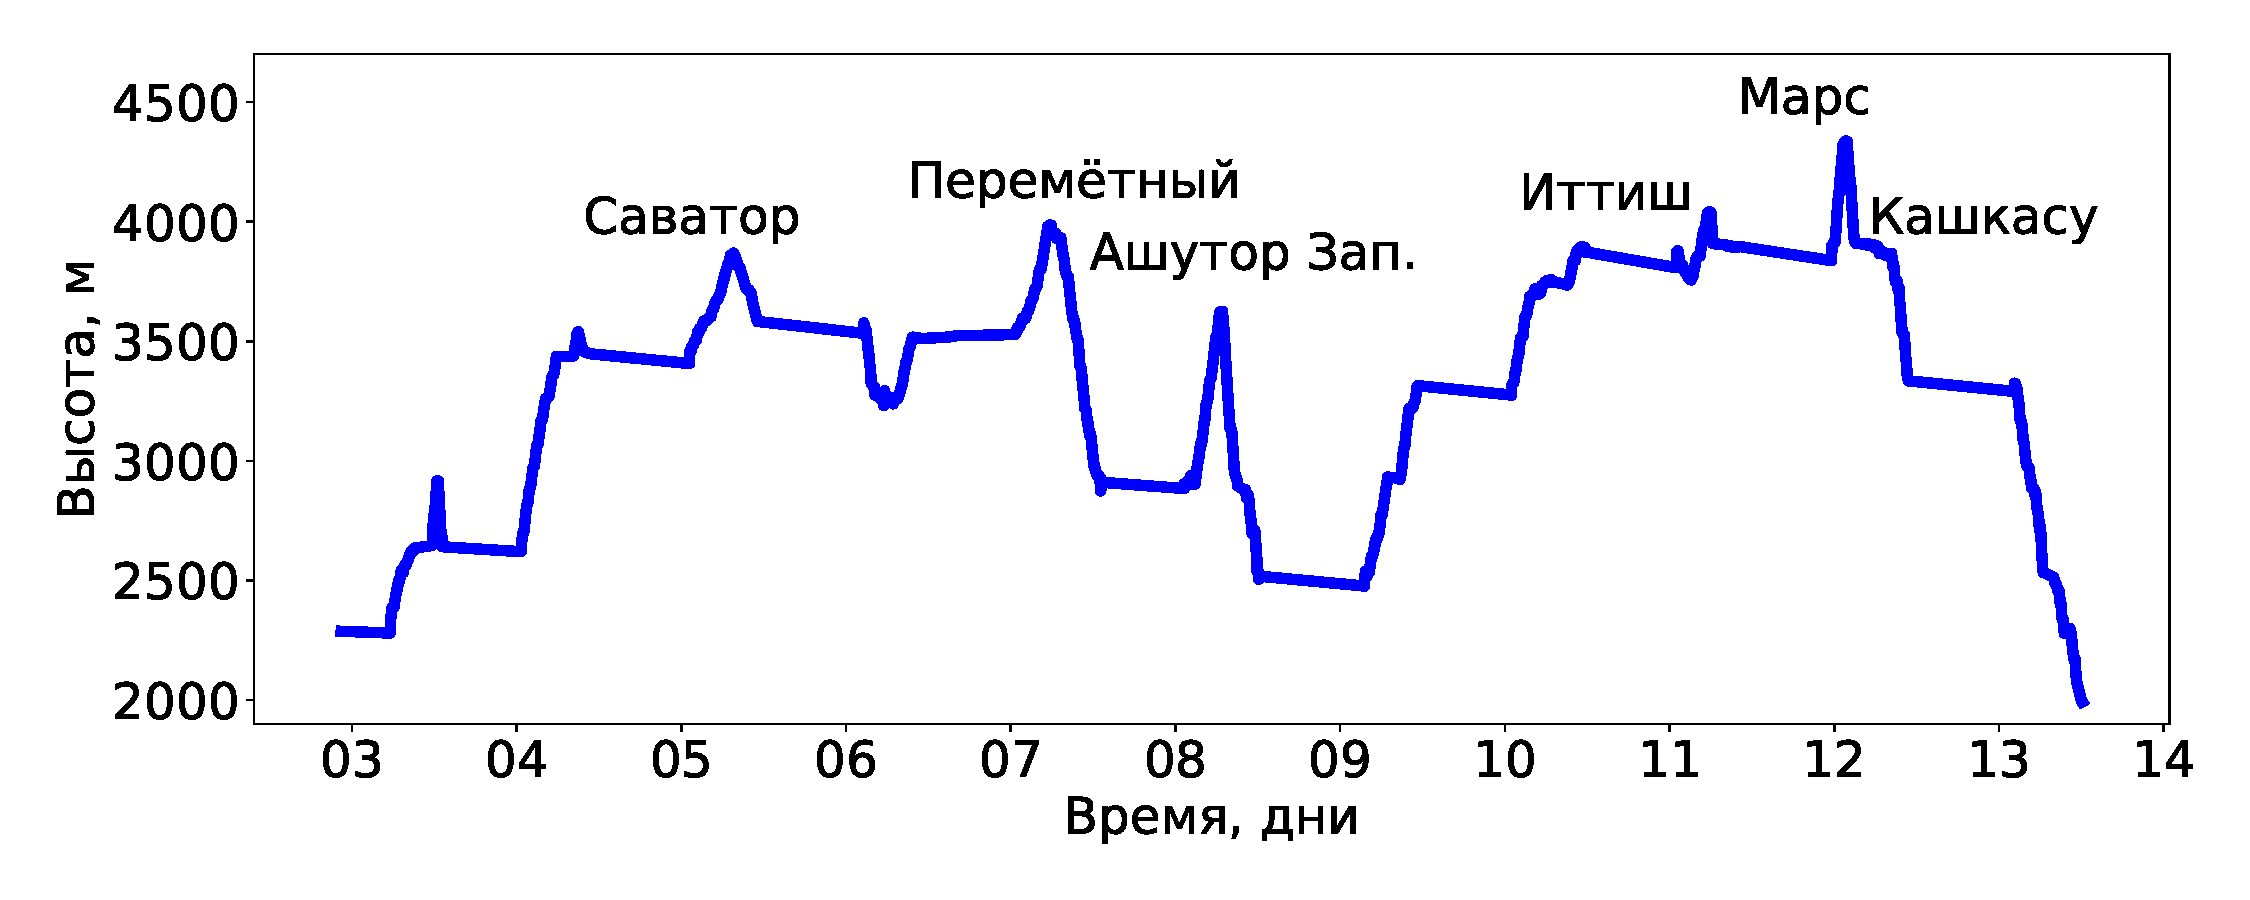
\includegraphics[width=0.92\linewidth]{pics/elevation_vs_time}
	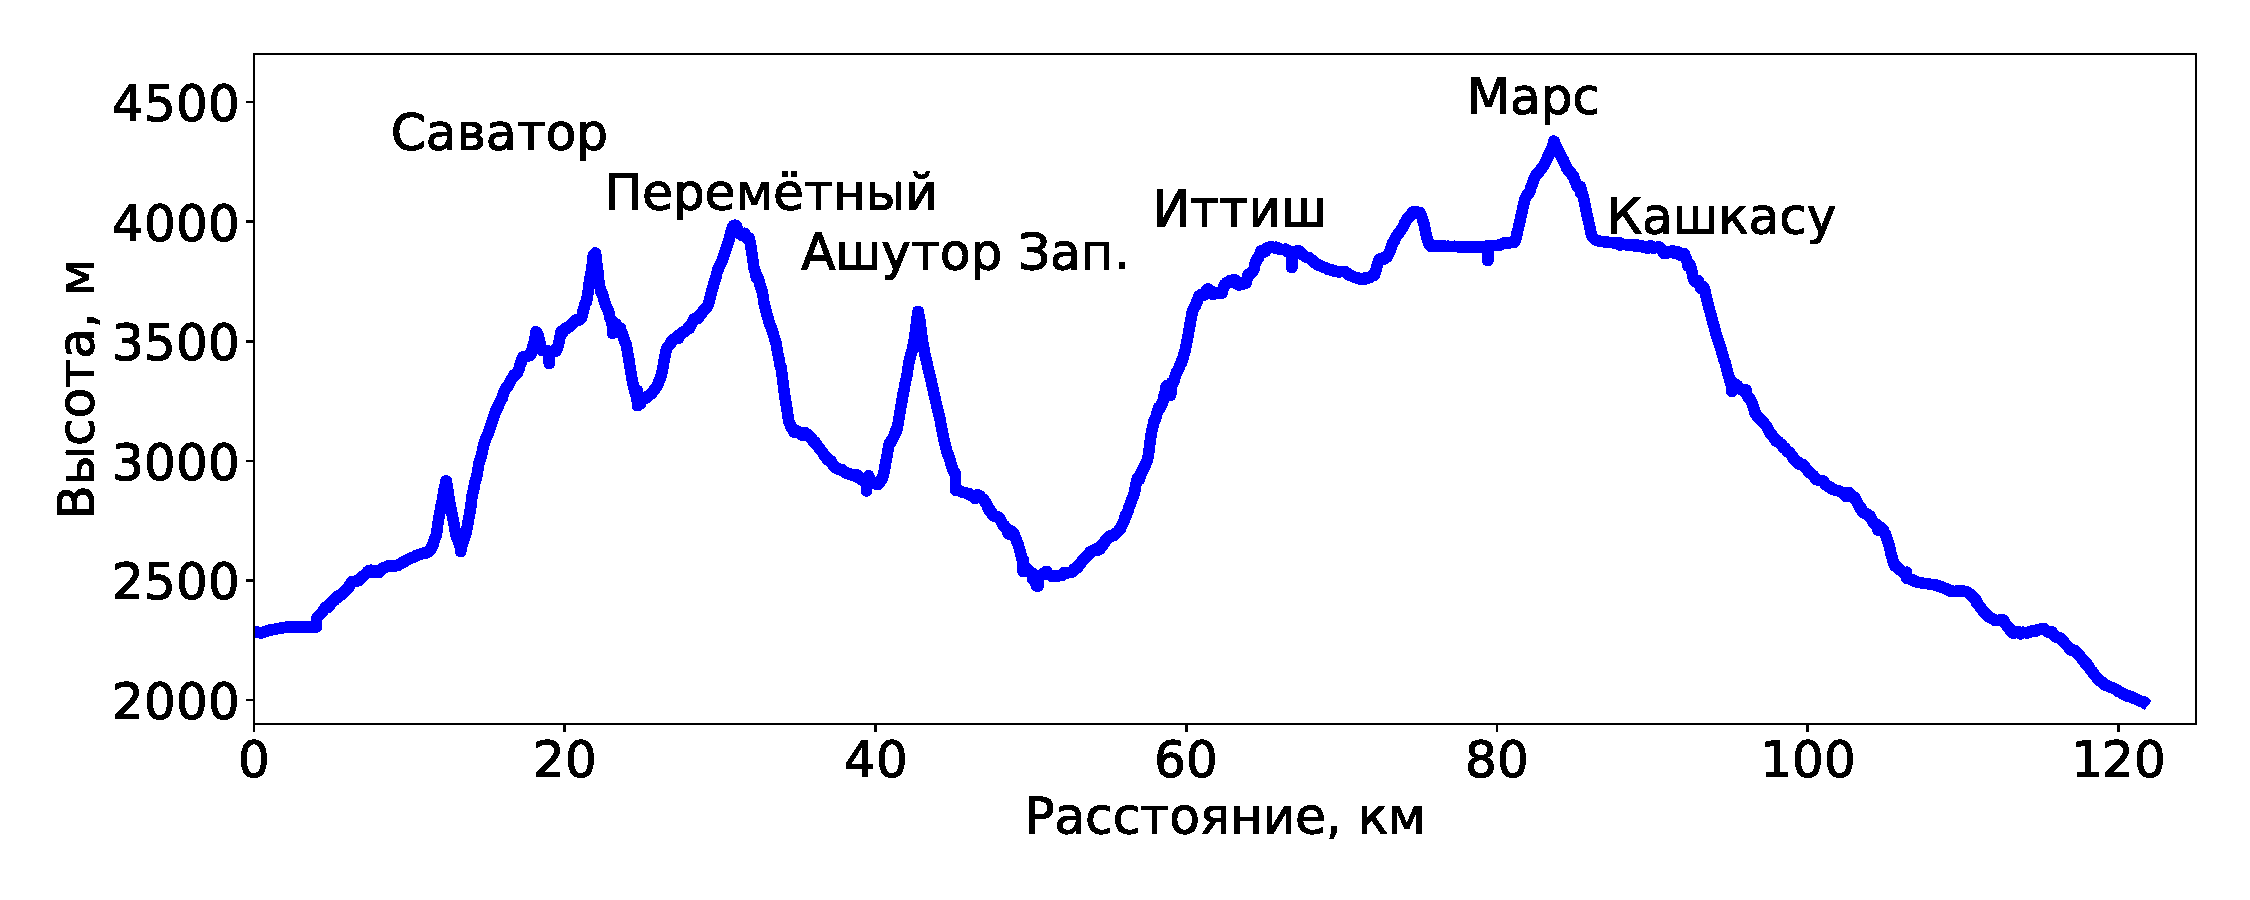
\includegraphics[width=0.92\linewidth]{pics/elevation_vs_distance}
	\caption{Высотный профиль маршрута}
	\label{fig:heights}
\end{figure}

\newpage
\subsection{Определяющие препятствия маршрута}

\begin{table}[h!]
		\begin{tabular}{|>{\centering\arraybackslash}m{0.17\linewidth}|>{\centering\arraybackslash}m{0.03\linewidth}|>{\centering\arraybackslash}m{0.35\linewidth}|>{\centering\arraybackslash}m{0.35\linewidth}|}
			\hline
			\textbf{Вид препятствия, высота} &
			\begin{turn}{90}\textbf{к. тр.}\end{turn} &
			\textbf{Характеристика препятствия на подъём} &
			\textbf{Характеристика препятствия на спуск} \\
			\hline			
			пер. Саватор (4000, по GPS~--- 3860) & 1А &  Со стороны д.р. Саватор тр.-ос. перевальный взлёт протяжённостью до 400 м и крутизной до $30^{\circ}$.  & Со стороны д.р. Киче-Кызыл-Суу ск.-ос., движение до $25^{\circ}$ и протяжённостью до 200 м по крупной и средней осыпи крутизной плотной группой, самостраховка ледорубами, далее~--- по гребню морены и моренному карману.\\
			\hline			
			пер. Перемётный, (4026)  & 1А & Со стороны д.р. Киче-Кызыл-Суу движение по моренному лабиринту, далее по моренным гребням выход на левый пхд борт ледника. Перемётный ледник длиной 1200 м и крутизной  до $15^{\circ}$, движение без кошек. & Движение по перемётному леднику до 300 м  крутизной  до $15^{\circ}$, далее по моренным валам, траверс мелкоосыпного склона протяжённостью до 2 км и крутизной  до $20^{\circ}$ \\
			\hline
			пер. Ашутор Западный (3700)  & 1А & Со стороны д.р. Джукучак по тр.-ос. склону по руслу пересохшего ручья протяжённостью до 300 м, крутизной до $15^{\circ}$, на перевальном взлёте до до $25^{\circ}$. & Движение по границе белой и чёрной мелких осыпей, далее по руслу пересохшего ручья протяжённостью до 150 м., крутизной до $20^{\circ}$\\
			\hline
			пер. Иттиш, (3895)  & 1А & Со стороны д.р. Иттиш движение по ос. гребню протяженностью до 700~м крутизной  до $15^{\circ}$ & Движение по тр. склону протяжённостью до 1000 м и крутизной до $5^{\circ}$\\
			\hline
			пер. Кашкасу, (3890)  & 1А & Со стороны озёр Кашкасу движение по дну ущелья протяжённостью до 2500 м без значительного уклона. &  Движение по гребням морен протяжённостью до 3500 м и уклоном до $15^{\circ}$\\
			\hline
	\end{tabular}%
\end{table}

\clearpage
\subsection{Список участников} 

\begin{table}[h!]
	\centering
	\resizebox{0.99\textwidth}{!}{%
	\begin{tabular}{|>{\centering\arraybackslash}m{0.015\linewidth}|>{\centering\arraybackslash}m{0.2\linewidth}|>{\centering\arraybackslash}m{0.18\linewidth}|>{\centering\arraybackslash}m{0.05\linewidth}|>{\centering\arraybackslash}m{0.15\linewidth}|>{\centering\arraybackslash}m{0.3\linewidth}|}
		\hline
		\textbf{№} &
		\textbf{Фото} &
		\textbf{ФИО} &
		\textbf{г.р.} &
		\textbf{Обязанности в группе} &
		\textbf{Туристский опыт} \\
		\hline			
		
		1	&	\includegoogle[width=0.99\linewidth]{https://drive.google.com/file/d/1WISFuT9mIPXXT3c39rQQxuTZFQ0DJDx6/view?usp=drive_link}	& Остапив Алексей Юрьевич	&	1998	&	Руководитель, завхоз, носитель аптечки	& 1ГР, Терскей\newline2ГУ, Киргизский хребет,\newline 3$\times$1ГУ, Кавказ, Алтай \newline 2А тур., 1Б альп.\\
		\hline
		2	&	\includegoogle[width=0.99\linewidth]{https://drive.google.com/file/d/1rtFU66LaAsBDkXLVvV_-qe-KaqowPTdq/view?usp=drive_link}	&	Миронова Наталья Сергеевна	&	2000	&	Логист, финансист	&	2 ст.с.  Кавказ\newline 1А тур.\\
		\hline
%		3	&	\includegoogle[width=0.99\linewidth]{https://drive.google.com/file/d/14mMi30ReTcrAUe4Hq6GsIjTiF4xvJbe7/view?usp=drive_link}	&	Гурский Артур Антонович	&	2003	&	Штурман, завснар, реммастер	&	1ГУ Терскей\newline1ПУ Крым\newline 1А тур.\\
%		\hline
%		4	&	\includegoogle[width=0.99\linewidth]{https://drive.google.com/file/d/1mPloHi0eN2j-M4MDuHpngwGsX-CevGd7/view?usp=drive_link}	&	Зернина Юлия Алексеевна	&	2004	&	Фотограф, хронометрист	&	1ГУ Терскей\newline 1А тур.\\
%		\hline
%		4*	&	\includegoogle[width=0.99\linewidth]{https://drive.google.com/file/d/1bN6RrMDDclIQesFk1KIZdMmjUpg2gKt6/view?usp=drive_link}	&	Йошта	&	2022	&	Талисман команды	&	1ГУ Кавказ\newline 1А тур.\\
%		\hline
	\end{tabular}%
}
\end{table}


\clearpage

\subsection{Географическое положение района}

Район Тескей-Ала-Тоо (кырг. <<Пёстрые горы, обращённые от солнца>>)~--- это горный хребет, входящий в горную страну Центрального Тянь-Шаня. Тескей расположен к югу от озера Иссык-Куль, простираясь с запада на восток на 375 км. Средняя высота хребта около 4500 м, высшая точка достирает 5216 м (пик Каракольский).

Крупные узлы оледенения расположены в верховьях рек Чон-Кызылсуу, Джеты-Огуз, Каракол, Арашан, Ак-Суу и Тургень-Ак-Суу. В целом степень оледеления обусловлена высотой и наличием влажного воздуха от Иссык-Куля.

При движении с запада на восток среднегодовое количество осадков увеличивается вдвое, с 1000 мм до 2000 мм (для высокогорья) \cite{rodina2012}. Температура воздуха колеблется летом от -5\degree (сырты, высота 4000 м, август) до 15\degree~(д.р. Джукучак, высота 2500 м, август)

В районе ярко выражена высотная поясность. Зона леса, представленная преимущественно высокими тянь-шаньскими елями, располагается на высотах 2100--3100 м. До высоты 3800 м следует зона альпийских лугов, а снеговая линия в августе находится на высотах от 4000 м (для северных склонов хребта). Южная же сторона хребта представлена заболоченным плоскогорьем~--- сыртами, и как по климату, так и по растительности и рельефу резко контрастирует с северной стороной.

Долины рек, текущих вдоль отрогов главного хребта, широкие, долины их боковых притоков узкие с высокой и крутой устьевой ступенью.

\subsection{Туристские особенности района}
Район очень привлекателен для горных туристов, поскольку в нём представляется возможным проведение горных походов любой к.с.~--- от <<единичек>> до <<шестёрок>>. Этому способствуют несколько факторов: достаточно простая логистика, наличие локальных препятсивий любого уровня сложности в достаточном количества, разнообразие природного рельефа. Уникальной особенностью западной оконечности центрального Тескея (долины рек Джууку, Иттиш, Ашукашкасу, Джукучак) является возможность перехода с северной стороны хребта на южную по перевалам с категорией сложности не выше 1А, чем строго рекомендуется пользоваться при планировании простых горных походов по району.

Самыми посещаемыми долинами являются д.р. Чон-Кызыл-Суу, Джеты-Огуз, Телеты, Каракол. Здесь, помимо спортивных, проходит множество коммерческих маршрутов, можно встретить туристов из Европы и США. Прочие долины, несмотря на хорошую изученность, посещаются значительно реже. Впрочем, стоит отметить сильно возросший интерес к д.р. Джууку, Иттиш, Ашукашкасу, Джукучак после публикации отчёта Д. Ковинова в 2021 году \cite{kovinov2021}.

К дополнительным особенностям района стоит отнести наличие горячих радоновых источников в д.р. Джеты-Огуз, Джукучак.

Типичной погодой для района следует считать ясную теплую первую половину дня и дождливый вечер (как правило, после 15:00) \cite{rodina2012, tipsina2024, sergeev2024, smurov2024}. Это следует обязательно учитывать при планировании ходового дня.

Все долины крупных рек, а также значительная часть их больших боковых притоков используются под высокогорных пастбища со всеми вытекающими последствиями для качества сырой воды.

\clearpage
	\section{Организация и проведение похода}
\subsection{Цели и задачи маршрута. Выбор нитки маршрута}
При разработке и планировании маршрута я, как руководитель, руководствовался следующими соображениями:
\begin{enumerate} 
	\item \textbf{Высотность, транспортная доступность горного района и стоимость трансфера.}
	Подавляющая часть группы (шесть человек из восьми) имела официальный или неофициальный опыт горных походов до 2 к.с по Кавказу \cite{Snegovskaya2024} или Алтаю, и вся группа имела высотный опыт ночёвки не менее 2900 м \cite{ostapiv2025}. Это позволило выбрать в качестве района новичкового похода не Гвандру или Архыз, как это обычно бывает, а новый для участников и руководителя горный район Центральной Азии~--- Тескей-Ала-Тоо. Высоты в этом районе, в среднем, на 500 м больше, чем на Кавказе, а его транспортную доступность можно назвать приемлемой для новичковых походов: 4 часа самолётом до Бишкека и еще 7~--- до места старта в горах. Стоимость трансфера выше, чем на Кавказе, но ниже, чем на Алтае. 
		
	\item \textbf{Концентрированность препятствий.}
	Дополнительным фактором в сторону выбора Тескей-Ала-Тоо послужило также и то, что в отличие, например, от Алтая, хребтовка района (основной хребет и серия параллельных отрогов), как и на Кавказе, позволяет осуществить подход под многие перевалы в течение одного дня, миновав долгие и занудные забеги по долинам, и, как следствие, поддерживать интерес группы на приемлемом уровне.
	
	\item \textbf{Разнообразие рельефа.} 
	С методической точки зрения, а также, опять-таки, для поддержания интереса группы, хотелось продемонстрировать участникам как можно больше разнообразных типов рельефа. Район позволяет в походах 1 к.с. продемонстрировать все виды рельефа, за исключением, пожалуй, снежного. <<Изюминкой>> района является возможность пересечения главного хребта через перевалы 1А (разительно отличающихся от классических <<единичек А>>) с осмотром высокогорных болот~--- сыртов.
	
	\item \textbf{Эффект кульминации.}
	У меня как у руководителя было глубокое убеждение, что первый поход должен обладать понятным, с позволения сказать, сюжетом и иметь свою кульминацию. В нашем случае таким сюжетом было движение через отроги главного хребта с преодолением разнообразных перевалов (последовательно: травянисто-осыпной, ледовый, травянистый), а затем~--- кольцо через главный хребет с <<неклассическими>> перевалами на южную сторону, восхождением на обзорную точку~--- вершину Марс. Конец маршрута~--- забег по среднегорью с финишем на локальной достопримечательности <<Красные скалы>>~--- также должен был добавить в поход разнообразия и красоты. Наконец, по моему глубокому убеждению, финальным аккордом походов по Кыргызстану должен быть хотя бы  однодневный (а лучше двухдневный) отдых на Иссык-Куле.
	
	\item\textbf{Помощь в планировании}
	Фактор, который формально не был в списке определяющих критериев, но по факту являлся таковым~--- это искренняя заинтересованность и помощь в планировании и организации маршрута от человека, через которого организовывалась логистика похода~--- Юрия Траченко. За эту помощь выражаю ему огромную благодарность.
	
\end{enumerate} 
\subsection{Логистика}
Подъезд осуществлён на поезде 033М Москва--Владикавказ до станции Минеральные Воды (прибытие в 03:40). Стоимость проезда на август 2024 г. составляла 7800~\faRub, купе (обратно – 4700~\faRub, плацкарт). От Минеральных Вод до аула Верхний Учкулан (время в пути 4 часа) добирались на трансфере, заказанном через Саракуева Бориса (89289503868, 89298843175,  \href{mailto: bezonec@list.ru}{bezonec@list.ru}). Стоимость трансфера трансфера туда составила 18000~\faRub, обратно (от поляны Азау) — 15000~\faRub. Стоимости доставки забросок в т/б Глобус и а/л Узункол составили 4000~\faRub~и 6000~\faRub.
Коллективный пропуск в пограничную зону КЧР был оформлен за 4 месяца до начала похода через электронную почту пограничного управления ФСБ по КЧР~--- \href{mailto: pu.kcherkes@fsb.ru}{pu.kcherkes@fsb.ru} и отправлен письмом по указанному адресу. Пропуск в КБР не требуется, так как пер. Хотютау в 2023 году был исключён из пограничной зоны \cite{order_kbr}.
\subsection{Аварийные выходы из маршрута и его запасные варианты}
\textbf{Аварийными выходами} с маршрута являлись:
\begin{itemize}
	\item На первом этапе: спуск к т/б <<Глобус>>;
	\item На втором этапе: спуск к а/л <<Узункол>>;
	\item На третьем этапе: спуск к погранзаставе <<Актюбе>> (Хурзук).
\end{itemize}
\textbf{Запасными вариантами} маршрута являлись:
\begin{itemize}
	\item Замена пер. Уллу-Кёль Восточный (1А$^\star$, 3050) на пер. \textbf{Уллу-Кёль Нижний (н/к, 2933)};
	\item Отказ от пер. Перемётный (1А, 3255), спуск по д.р. Чунгур-Джар;
	\item Отказ от пер. Хотютау (1А$^\star$), спуск по д.р. Кубань к погранзаставе <<Хурзук>>
\end{itemize}
\subsection{Изменение маршрута и их причины}
Воспользовались запасным вариантом~--- отказ от прохождения пер. Сылтран и спуск в Верхний Баксан по д.р. Кыртык. Сделали это в связи с тем, что длительный спуск (около 2 км по вертикали) почти гарантированно привёл бы к проблемам с коленями у одного из участников. К тому же, судя по отзывам встреченных нами туристов, на седловине перевала уже лежал снег.
\subsection{Обеспечение безопасности на маршруте}
Группа была зарегистрирована в отделении МЧС Кыргызстана по Иссык-Кульской области (телефон +996555004214, связь по WhatsApp). За 10 дней до похода были переданы сведения о составе группы, сроках и маршруте, в ответ был получен регистрационный номер и просьба проинформировать дежурного о начале и завершении похода.

\alert{Дима, это с тебя Для регулярного обмена сообщениями, отслеживания положения группы на карте, а также возможности экстренной связи, в группе имелся спутниковый треккер IRIDIUM Rockstar 360. Стоимость аренды треккера в <<Альпиндустрии>> на 15--21 день составила 7100~\faRub, залог~--- 50000~\faRub. Нам повезло попасть на демострационный период тарифа треккера, в связи с чем все сообщения были для нас безлимитны и бесплатны. Предварительное тестирование треккера в Москве показало, что спутниковые сигналы в столице эффективно глушатся: сообщения приходили не чаще раза в сутки. В походе с приёмом и отправкой сообщений и координат на сервер проблем не возникало, среднее время отправки составляло 30 минут.}

Каждый участник самостоятельно оформлял на себя индивилуальный страховой полис. Выбрали страховую фирму <<Согласие>>, ассист Balt Assistance, опция <<Треккинг свыше 1500 м>>, размер страховой защиты 35000~USD,  вид отдыха <<Спорт Экстрим>>. Стоимость полиса составила 8234~\faRuble~с человека.

\subsection{Перечень наиболее интересных природных и исторических объектов, занятий на маршруте}
\begin{enumerate}[noitemsep,topsep=0pt,parsep=0pt,partopsep=0pt]
	\item Широкие красивые долины северной стороны хребта: Чон-Кызыл-Суу, Киче-Кызыл-Суу, Ашукашкасу, Джукучак; 
	\item Сырты на южной стороне хребта; 
	\item Цепочка озёр Кашкасу с чистой водой; 
	\item Вершина Марс, с которой открываются виды на Акширак, Кумтор, сырты и, в хорошую погода, на семитысячники; 
	\item Перевал Кашкасу, через который в былые годы перегоняли лошадей. Следы этого остаются в ущелье до сих пор, жутковато и атмосферно; 
	\item <<Красные скалы>> на слиянии р. Джууку и Джукучак;
	\item Иссык-Куль.
\end{enumerate}

\paragraph{Темы практических занятий:}

\begin{itemize}
	\item Техника передвижения по травянистым и осыпным склонам;
	\item Техника несложных бродов поодиночке;
	\item Техника передвижения по льду.
\end{itemize}

\newpage
\subsection{Развёрнутый график движения}
\alert{Дима, это на тебе, пожалуйста}
\begin{table}[h!]
	\centering
	\resizebox{0.95\textwidth}{!}{%
		\begin{tabular}{|>{\centering\arraybackslash}m{0.045\linewidth}
				|>{\centering\arraybackslash}m{0.02\linewidth}
				|>{\centering\arraybackslash}m{0.43\linewidth}
				|>{\centering\arraybackslash}m{0.09\linewidth}
				|>{\centering\arraybackslash}m{0.1\linewidth}
				|>{\centering\arraybackslash}m{0.05\linewidth}
				|>{\centering\arraybackslash}m{0.09\linewidth}
				|>{\centering\arraybackslash}m{0.13\linewidth}|}
			\hline						
			Дата	&	\begin{turn}{90}День\end{turn}	&	Участок маршрута	&	Км с $k=1.2$	&	Набор /сброс, м	&	ЧХВ	&	Высота ночёвки, м	&	Способы передвижения	\\
			\hline
			
			18.08	&	1	&	г.~Минеральные воды~--- аул Верхний Учкулан~--- д.р Учкулан~--- д.р. Кичкинакол Уллукёльский	&	5.3	&	$+650$\newline$-0$	& 2:46	&	2200	&	Машина,\newline Пешком	\\
			\hline
			19.08	&	2	&	д.р. Кичкинакол Уллукёльский~--- оз. Гитче-Кёль~--- оз. Уллу-Кёль 	&	5.6	& $+650$\newline$-0$		& 3:25		& 2850		&	Пешком	\\
			\hline
			20.08	&	3	&	м.н.~--- \textbf{пер. Уллу-Кёль Восточный (1А$^\star$, 3050)}~--- кош в д.р. Трёхозёрная~--- д.р. Махар	&	7.2	& $+200$\newline$-1190$		& 7:39	& 1860		&	Пешком	\\
			\hline
			21.08	&	4	&	м.н.~--- т/б <<Глобус>>~--- д.р. Гондарай~--- д.р. Джалпаккол	&	11.3	&$+390$\newline$-225$		& 3:54		& 2120		&	Пешком	\\
			\hline
			22.08	&	5	&	м.н.~--- д.р. Кичкинекол Джалпаккольский~--- м.н. под моренным валом пер. Джалпаккол Северный	&	5.8	& $+620$\newline$-0$		& 3:56	& 2740		&	Пешком	\\
			\hline
			23.08	&	6	&	м.н.~--- \textbf{пер. Джалпаккол Северный (1А$^\star$, 3411)}~--- зелёные ночёвки на спуске в д.р. Мырды	&	5.0 	& $+660$\newline$-395$		& 6:16		& 3015		&	Пешком	\\
			\hline
			24.08	&	7	&	м.н.~--- д.р. Мырды~--- а/л <<Узункол>>	&	7.5	& $+0$\newline$-960$		& 3:53		& 2060		&	Пешком	\\
			\hline
			25.08	&	8	&	м.н.~--- д.р. Кичкинекол~--- д.р. Таллычат~--- Поляна Крокусов	&	7.1	& $+780$\newline$-0$		& 3:23		& 2840		&	Пешком	\\
			\hline
			26.08	&	9	&	м.н.~--- \textbf{пер. Кичкинекол Малый (1А, 3206)}~--- д.р. Чунгур-Джар	&	4.6	& $+360$\newline$-520$		& 2:42		& 2680		&	Пешком	\\
			\hline
			27.08	&	10	&	м.н.~--- \textbf{пер. Перемётный (1А, 3255)}~--- д.р. Танышхан	&	7.1	& $+575$\newline$-935$		& 6:50		& 2320		&	Пешком	\\
			\hline
			28.08	&	11	&	м.н.~--- д.р. Чиринкол~--- д.р. Кубань &	12.7	& $+90$\newline$-500$		& 3:23		& 1890		&	Пешком	\\
			\hline
			29.08	&	12	&	м.н.~--- погранзастава <<Хурзук>>~(рад.)~--- д.р. Уллу-Кам	&	20.9	& $+1210$\newline$-370$		& 7:15		& 2725		&	Пешком	\\
			\hline
			30.08	&	13	&	м.н.~--- \textbf{пер. Хотютау (1А$^\star$, 3546)}~--- лед. Большой Азау~--- оз. Эльбрусское~--- ст. <<Старый Кругозор>>~--- поляна Азау & 10.9	& $+800$\newline$-615$		& 4:25		& 2915		&	Пешком, Канатная дорога	\\
			\hline
			\multicolumn{3}{|c|}{\textbf{\textit{\Large{Итого:}}}} & \large{\textbf{111.0}} & \large{$\mathbf{+6985}$\newline$\mathbf{-5210}$	}	& \multicolumn{3}{c|}{\large{\textbf{58:08}\newline\textbf{2д 10ч 08мин}}} \\
			\hline
		\end{tabular}
}	
	
\end{table}



\clearpage
%	\section{Литературный обзор по прохождению маршрута}

\subsection{Пер. Иттиш}

Пер. Иттиш ориентирован с севера на юг и является перевалом через основной хр. Тескей-Ала-Тоо. Это один из немногих перевалов (наряду с пер. Кашкасу, Джукучак) через данный основной хребет, которые имеют (низкую) трудность 1А. Вообще говоря, пер. Иттиш~--- это выход на горизонтальное плато, на котором расположены сырты (заболоченные луга). Лишь северная сторона перевала имеет наклон. Перевал чаще проходится с юга на север \cite{kovinov2021,sergeev2024,tipsina2024}; в данном походе было решено преодолеть его на подъём с севера на юг. При подготовке использовались отчёты \cite{kovinov2021,sergeev2024,tipsina2024}, также о возможности проходения перевала в обратную сторону руководитель узнавал у Натальи и Григория по почте.

Подъём на перевал можно разбить на две части: подъём по тропе по хвойному лесу и осыпи и горизонтальное движение по средней и крупной осыпи. Второй этап недлинный по расстоянию~--- около 4--5 км~--- но может занять много времени из-за трудности рельефа. В некоторых местах можно сойти с крупных камней и двигаться по пересохшему дну озер, находящихся вблизи осыпи. При подходе к седловине видно обледенелый пик Иттиш и ледник, примыкающий к нему (цирк пер. Иттиш Левый (2А)). После взятия перевала спуска нет~--- сразу идёт выход на высокогорные сырты и озёра. В хорошую погоду с седловины открывается вид на соседний хр. Акшийрак. В целом, подъём является постепенным и не имеет крутых взлётов.

Суммарный перепад высот от д.р. Джууку, из которой начинался подъем, до седловины перевала составляет около 1000Ём, поэтому было решено устроить ночёвку в середине подъёма на небольшом озере, находящимся выше границы леса на высоте 3300~м. От м.н. на озере до седловины перевала был пройден остаток подъёма по средней осыпи и затем преодолен упомянутый затяжной участок горизонтальной крупной осыпи.

\clearpage
	\section{Техническое описание маршрута}
\textit{Примечание:} везде, если не оговорено иное, имеются в виду правые и левые берега рек \textbf{орографически}.

\textbf{Отчёт писали:} Наташа Миронова, Лёша Остапив.
\subsection{05 августа. Старт}
\textit{Метеоусловия: ясно}

\begin{figure}[h!]
	\centering
	\includegraphics[angle=90, width=0.5\linewidth]{pics/maps/05}
	\label{fig:05}
\end{figure}

Приезжаем на место старта~--- в а. Хурзук~--- в 18:30. На улице уже глубокие сумерки, переходящие в ночь.

\begin{figure}[h!]
	\centering
	\includegraphics[width=0.6\linewidth]{pics/_DSC0007}
	\caption{Вечерний Хурзук}
	\label{fig:_DSC0007}
\end{figure}

Фонарики далеко не убираем, выдвигаемся по д.р. Уллухурзук по хорошей автомобильной дороге. По пути встречаем команду мотоциклистов из Краснодара, которые планируют кататься в этих же краях. За 40 мин ЧХВ доходим до д.р. Еникол и встаём на ночёвку на отличной оборудованной площадке. Коорлинаты м.н.: N 43.42806° E 42.18472°.

\clearpage
\subsection{06 сентября. д.р. Енукол, пер. Енукол}
\textit{Метеоусловия: весь день ясно, солнечно}

\begin{figure}[h!]
	\centering
	\includegraphics[angle=0, width=0.45\linewidth]{pics/maps/06}
	\label{fig:06}
\end{figure}

Подъём в 06:00. Завтракаем, распределяес еду и снарягу и в 07:50 выдвигаемся в путь.

\alert{ФОТКА ЛАГЕРЯ}

За первые 30 мин ЧХВ выходим по дороге из зоны леса. Нас обгоняют вчерашние мотоциклисты и уезжают в сторону перевала. Немного выше зоны леса (2150 м) дорога заворачивает налево пхд к кошу, мы же поднимается по руслу пересыхающего ручья~--- правого притока р. Енукол. Подъём технически несложный, но отсутствие дорог и человеческих (коровьи -- в количестве) сказывается на скорости движения. Впрочем, в 11:05, к общей радости, мы выходим на дорогу у оборудованного родника (N 43.44810° E 42.21287°).

Дальнейшее движение не представляет сложности, ибо основной набор высоты позади. Идём по дороге, в 12:25 выходим на седловину пер. Енукол. Отгоняем Йошту от собаки пастуха, что пасёт здесь лошадей.

\alert{ФОТКА С ПЕРЕВАЛА}






\clearpage
\subsection{07 августа. пер. Быкылы, пер. Чемарт}
\textit{Метеоусловия: }

\begin{figure}[h!]
	\centering
	\includegraphics[angle=90, width=0.8\linewidth]{pics/maps/07}
	\label{fig:07}
\end{figure}



\clearpage
%\subsection{08 августа. пер. Бурунташ, а/л <<Лакколит>>}
\textit{Метеоусловия: ночью дождь, утром переменная облачность, ясно, днём, вечером, ночью дождь}

\begin{figure}[h!]
	\centering
	\includegraphics[angle=90, width=0.8\linewidth]{pics/maps/08}
	\label{fig:08}
\end{figure}

Начиная с 04:00 сквозь сон мониторим обстановочку. Встаём в 05:00, как только прекращается дождь. Завтракаем, любуемся свежим снегом на вершинах (запорошило склоны выше приблизительно 3500~м). Выходим в 06:25 и движемся по тропе вдоль правого притока р. Чемарткол в сторону пер.~Бурунташ. Кажется, что в этих краях коровки--биологические газонокосилки не ходят, поэтому тропа норовит скрыться в мокрой траве (рис.~\ref{fig:burun_river}).

\begin{figure}[h!]
	\centering
	\includegoogle[width=0.8\linewidth]{https://drive.google.com/file/d/1qrRYZxMfuf8lq3XnpOfDnIqa0ttqPWRv/view?usp=drive_link}
	\caption{Подъём на пер. Бурунташ}
	\label{fig:burun_river}
\end{figure}

Затем тропа заворачивает налево пхд, обходя небольшой прижим. Здесь на протяжении 200 горизонтальных метров даже есть ощутимый уклон до 20\degree. 

\begin{figure}[h!]
	\centering
	\includegoogle[width=0.7\linewidth]{https://drive.google.com/file/d/1e0Niv_SpAj9JCnEIDDpLY4pJaek7L2Nt/view?usp=drive_link}
	\caption{Подъём на пер. Бурунташ}
	\label{fig:burun_uphill}
\end{figure}


Однако далее, чем ближе к седловине, тем более тропа напоминает скоростное шоссе, идущее, причём, по обоим берегам ручья. В целом, тропа на пер. Бурунташ показалась достаточно интересной именно из-за своего разнообразия.

\begin{figure}[h!]
	\centering
	\includegoogle[width=0.7\linewidth]{https://drive.google.com/file/d/1ZbswaeJXmXBv1cY8FkzUNN5LK-6zX6Wb/view?usp=drive_link}
	\caption{Подъём на пер. Бурунташ}
	\label{fig:burun_uphill_1}
\end{figure}

По дороге (N 43.42597°, E 42.41327°) видим несколько мест для ночёвки. Воды много.


На седловину пер. Бурунташ выходим в 08:35. Она представляет собой очень широкое плато, на котором, поначалу, даже непонятно, где искать перевальный тур. Находим его около большого камня с памятной табличкой, установленной в 2025 году в честь годовщины победы в ВОВ, координаты: N 43.42390° E 42.42623°. К сожалению, вокруг много лже-туриков с мусором внутри \frownie. Погода ясная, вид на Эльбрус и окрестности потрясающий. Устраиваем фотосессию на фоне горы.

\begin{figure}[h!]
	\centering
	\includegoogle[width=0.7\linewidth]{https://drive.google.com/file/d/1uoUO_yBKoYSdvhsErMBe_y_Mrm1I_joE/view?usp=drive_link}
	\caption{пер. Бурунташ, вид на Эльбрус}
	\label{fig:buruntash1}
\end{figure}

\begin{figure}[h!]
	\centering
	\includegoogle[width=0.7\linewidth]{https://drive.google.com/file/d/1YDXBwDvdmo66RN5_xplST0r_Vy_PMBWZ/view?usp=drive_link}
	\caption{пер. Бурунташ, вид в долину правого притока Чемарткола (путь подъёма)}
	\label{fig:buruntash2}
\end{figure}

В 9:15 начинаем спуск. С восточной стороны склон также пологий и по нему идут несколько троп. По одной из них в 10:03  спускаемся к р.~Кызылкол (карач.-балк. \textit{<<Красное ущелье>>}). Мы знаем, что на точке N 43.42654° E 42.43766° должен быть натянут трос для переправы, но знаем также, что, судя по отзывам туристов этого сезона, в количестве присутствуют места, в которых реку можно перейти по камням. Одно из таких мест находим здесь: N 43.42483° E 42.43703°. Сомнения вызывает только шаг с предпоследнего камня на последний. На всякий случай делаем этот шаг без рюкзаков, которые предварительно бросаем на целевой берег (речь идет о расстоянии около метра, так что упустить рюкзак в воду было бы сложно). На всё про всё у наш ушло меньше 7 минут.

\begin{figure}[h!]
	\centering
	\includegoogle[width=0.9\linewidth]{https://drive.google.com/file/d/1MtaAatVQGYh2Eem3x5S_7JmeE5qXaUbz/view?usp=drive_link}
	\caption{Слева: самцы в напряге (передача более длинных палок); по центру и справа: переправа последнего участника}
	\label{fig:pereprava}
\end{figure}

Далее нам необходимо забраться на плато Ирахиксырт. Для этого можно двигаться по тропе, спустившись вдоль реки на 40 вертикальных метров, а затем набрав около 100 м по склону. Мы хотим сэкономить паразитный сброс и движемся траверсом по склону в надежде в дальнейшем подрезать тропу. Однако надежды оказались напрасны: мы вырулили прямо на небольшой распадок и всё-таки были вынуждены организовать паразитный сброс. Зато потренировали спуск по травянистому склону с использованием альпенштока и движение плотной группой.

\begin{figure}[h!]
	\centering
	\includegoogle[width=0.4\linewidth]{https://drive.google.com/file/d/1lBvIVKY6-MzG7B5uPtWJXVRbOdTQjTe0/view?usp=drive_link}
	\caption{Тренировка спуска по травянистому склону с использованием альпенштока и движения плотной группой}
	\label{fig:trenya}
\end{figure}



Так или иначе, к 11:00 таки выходим на плато, любуемся открывшимися видами и интересными минеральными выходами на склонах левого берега р.~Кызылкол.

\begin{figure}[h!]
	\centering
	\includegoogle[width=0.9\linewidth]{https://drive.google.com/file/d/1KizZE64GMWdahdubWcXPDyvJi-6d59Ps/view?usp=drive_link}
	\caption{Панорама плато Ирахиксырт, вид на восток}
	\label{fig:plauteau}
\end{figure}

По плато идёт отличная тропа, без проблем пересекаем его и подходим к м.н.~--- а/л <<Лакколит>>. Перед спуском с плато ловим связь и мобильный интернет (редкость в наше время!) у оператора <<Мегафона>> (и у <<Tele2>>, который поймал вышку первого).

\begin{figure}[h!]
	\centering
	\includegoogle[width=0.9\linewidth]{https://drive.google.com/file/d/1Sq8n4ApW8FN0YOp8Ivcp2r6GiudJT4-B/view?usp=drive_link}
	\caption{Спуск с плато, вид в сторону Джилы-Су}
	\label{fig:lakkolit}
\end{figure}

\begin{figure}[h!]
	\centering
	\includegoogle[width=0.9\linewidth]{https://drive.google.com/file/d/1cYX3GR8wBCrL91uHwuEJXRGMFmWCdKg9/view?usp=drive_link}
	\caption{Спуск с плато, вид в сторону плато Ирахиксырт. Фото сделано утром следующего дня}
	\label{fig:lakkolit2}
\end{figure}

В 13:00 спускаемся к альплагерю и встаём лагерем. За 500~\faRub~с человека в нашем распоряжении общественная палатка со столами и скамьями для готовки еды и уборная. Горячий душ стоит 400~\faRub~с человека. Как только становимся лагерем~--- начинается мелкий дождь, который с переменным успехом идёт до 07:00 следующего дня. От альпинистов узнаём плохой прогноз погода на следующие двое суток. Прямо как в <<Метеорологии>> Смешариков~--- <<Дождь будет идти ещё сорок восемь часов>>.

ЧХВ: 4:30, ОХВ: 6:15

Координаты м.н.: N 43.42947° E 42.51142°.

\clearpage
%\subsection{07 августа. пер. Перемётный (1А)}
\textit{Метеоусловия: утром, днём ясно, с 15:00 по 19:00 пасмурно, дождь, ночью сильный дождь}

\begin{figure}[h!]
	\centering
	\includegraphics[angle=90, width=0.7\linewidth]{pics/maps/07}
	\label{fig:07}
\end{figure}

Подъём дежурных в 04:30, выход в 07:10. Движемся к левому берегу одного из притоков в сторону небольшого голубого озерца в течение 15 мин ЧХВ и подходим к подножию морен. Приток можно перейти по камням, некоторые участники переходят в бродовой обуви.

\begin{figure}[h!]
	\centering
	\includegraphics[width=0.7\linewidth]{pics/07/IMG_2778}
	\caption{Место брода и дальшейшее движение по морене}
	\label{fig:img2778}
\end{figure}

Далее забираемся на моренный вал, огибаем локальную возвышенность справа пхд (рис.~\ref{fig:img2778}) и следуем по локальному понижению в направлении цирка Лавинных перевалов в течение 30 мин ЧХВ. Уклон не более 15\degree, подниматься комфортно (рис.~\ref{fig:DJI_0059.jpg}).

\begin{figure}[h!]
	\centering
	\includegraphics[width=0.9\linewidth]{pics/07/DJI_0059.jpg}
	\caption{Маршрут подъёма на пер. Перемётный}
	\label{fig:DJI_0059.jpg}
\end{figure}

Выходим на левый пхд борт ледника с осыпного гребня, разделяющего цирки Лавинных перевалов и пер. Перемётный, поскольку подъём с языка ледника без кошек невозможен. Сам же ледник открытый, пологий и проходится без кошек. Его уклон не превышает 10\degree, лишь в верхней части есть участок крутизной до 15\degree и с поперечными трещинами, которые легко обходятся.

\begin{figure}[h!]
	\centering
	\includegraphics[width=0.7\linewidth]{pics/07/IMG_2857.jpg}
	\caption{Движение по леднику}
	\label{fig:IMG_2857.jpg}
\end{figure}

\begin{figure}[h!]
	\centering
	\includegraphics[width=0.7\linewidth]{pics/07/IMG_2904.jpg}
	\caption{Движение по леднику}
	\label{fig:IMG_2904.jpg}
\end{figure}

\begin{figure}[h!]
	\centering
	\includegraphics[width=0.9\linewidth]{pics/07/view_kiche.jpg}
	\caption{Маршрут подъёма, вид с седловины}
	\label{fig:view_kiche.jpg}
\end{figure}

Движемся по леднику в течение 70 мин ЧХВ и в 11:30 выходим на перевал. Седловина~--- широкое ледовое плато, тура, как и писали в предыдущих отчётах, нет. Складываем свой тур на осыпном гребешке правого пхд борта перевала в надежде, что если группы будут ходить здесь каждый год, то он не будет успевать уезжать вместе с перемётным ледником. Координаты сложенного нами тура: N 42.09765° E 78.12405°.

\begin{figure}[h!]
	\centering
	\includegraphics[width=0.9\linewidth]{pics/07/DJI_0067.jpg}
	\caption{Группа на пер. Перемётный (1А). Вид в д.р. Джукучак}
	\label{fig:DJI_0067.jpg}
\end{figure}

\begin{figure}[h!]
	\centering
	\includegraphics[width=0.9\linewidth]{pics/07/DJI_0069.jpg}
	\caption{Группа на пер. Перемётный (1А). Вид в д.р. Киче-Кызыл-Суу}
	\label{fig:DJI_0069.jpg}
\end{figure}


\begin{figure}[h!]
	\centering
	\includegraphics[width=0.7\linewidth]{pics/07/typ.jpg}
	\caption{Местоположение перевального тура}
	\label{fig:typ.jpg}
\end{figure}

Спускаемся по пологому правому борту ледника до озера в течение 15 минут. Этот участок также проходим без кошек, но трое участников их всё же надевают, скорее, потому что кошки были в наличии. В крайнем случае при спуске есть возможность перейти на правый пхд осыпной борт и спуститься там.

\begin{figure}[h!]
	\centering
	\includegraphics[width=0.7\linewidth]{pics/07/IMG_2970.jpg}
	\caption{Путь спуска с пер. Перемётный}
	\label{fig:IMG_2970.jpg}
\end{figure}

За озером находятся галечные площадки (координаты: N 42.09315° E 78.11896°), на которых, при необходимости, можно встать на ночёвку. Вода из правого притока р. Джукучак, этот ручей как раз берет своё начало здесь. На этом месте мы обедаем и в 13:10 выдвигаемся на спуск. Ручей довольно быстро уходит в систему каньонов (насчитали три штуки), поэтому спускаемся, траверсируя склон правого борта притока. Под ногами мелкая осыпь, но она достаточно крупна, чтобы <<лифтом>> спускаться было не очень удобно. Двигаемся медленно и аккуратно, так как склон крутой и заканчивается каньоном. Кроме того, нам встречаются две селевые промоины, борта которых сцементированы прошедшим потоком. Первая промоина неглубока и перебраться через неё не составило труда, а для преодоления второй пришлось спуститься на 20~м, а потом подняться обратно.

\begin{figure}[h!]
	\centering
	\includegraphics[width=0.7\linewidth]{pics/07/IMG_3031.jpg}
	\caption{Траверс осыпного склона}
	\label{fig:IMG_3031.jpg}
\end{figure}

\begin{figure}[h!]
	\centering
	\includegraphics[width=0.9\linewidth]{pics/07/IMG_3041.jpg}
	\caption{Траверс осыпного склона (вид в сторону перевала)}
	\label{fig:IMG_3041.jpg}
\end{figure}

Далее идёт спуск по крутому (до 30\degree) травянистому склону. Здесь важно не уходить слишком вправо, хоть там склон и положе, так как этот пологий склон оканчивается скальными выходами. Сильно влево забирать также нельзя, так как река снова образует каньон.

\begin{figure}[h!]
	\centering	\includegraphics[width=0.7\linewidth]{pics/07/IMG_3087.jpg}
	\caption{Спуск по крутому тр. склону в <<коридоре>> между обрывом и скальными  выходами}
	\label{fig:IMG_3087.jpg}
\end{figure}


В 16:50 спускаемся, наконец, на дно д.р. Джукучак и движемся вниз по долине в направлении ночёвок под пер. Ашутор Зап. Спустя 30 минут движения нас накрывает дождём. Решаем вставать на первых же удобных площадках и бродить р. Джукучак утром следующего дня. В итоге выбираем место за 600 м до брода через р. Джукучак. Первые участники подходят под м.н. в 18:30, ставят палатки и греют чай. Остальные подтягиваются к 19:00, поим всех чаем и раскладываем отдыхать. Дежурные также разносят еду по палаткам. Дождь к вечеру прекращается, однако ночью льёт пуще прежнего.
Координаты м.н.: N 42.11030° E 78.05595°. ЧХВ 10:14.

\begin{table}[h!]
	\centering
	\begin{tabular}{|c|c|c|c|c|c|} 
		\hline 
		Этап & ЧХВ \\ 	
		\hline 
		Подъём в верховья р. Киче-Кызыл-Суу  & 02:00 \\
		Подход по моренам к леднику  & 03:00 \\
		По леднику до седловины & 01:10\\ 
		По леднику до галечных площадок & 00:50\\ 
		Траверс осыпного склона & 02:40\\ 
		Спуск по травянистому склону в д.р. Джукучак & 00:35 \\
		\hline
		\textsc{Полное время подъёма на перевал  }& 06:10\\
		\textsc{Полное время спуска с перевала }& 04:05 \\
		\textsc{	Полное время прохождения перевала }& 10:15 \\
		\hline
	\end{tabular}
	\caption{Расклад времени, пер. Перемётный}
\end{table}



\textbf{Выводы и рекомендации:} пер. Перемётный соответствует заявленной категории трудности 1А (при условии открытого ледника Киче-Кызылсу), достаточно красив и интересен. Подъём на перевал не представляет сложности, интересен распутыванием несложного моренного лабиринта и длинным пологим ледником. Последнее обстоятельство особенно ценно: не в каждом походе 1 к.с. удастся вдоволь погулять по леднику. Спуск по долине правого притока р. Джукучак долог и утомителен: сначала 2 км траверса малко-средней сыпухи, ведущей в ущелье каньона, затем~--- лавирование по достаточно крутому травянистому склону между скальными сбросами и ещё более крутым склоном. Для новичков такие препятствия могут быть выматывающими при прохождении, это нужно учитывать при планировании ходового дня. Перевал не рекомендуется ставить первой <<единичкой А>> на маршруте и проходить его в обратную сторону (с юга на север). 

\clearpage
%\subsection{08 августа. пер. Ашутор Западный}
\textit{Метеоусловия: }

\begin{figure}[h!]
	\centering
	\includegraphics[angle=0, width=0.7\linewidth]{pics/maps/08}
	\label{fig:08}
\end{figure}

\textit{Ашутор (кырг.)~--- <<Перевальное урочище>>}


\clearpage
%\subsection{11 сентября. Долина р.Кыртык, финиш}
\textit{Метеоусловия: утром туман, к полудню развиднелось, после солнечно.}

%\begin{figure}[h!]
%	\centering
%	\includegraphics[width=0.7\linewidth]{pics/09/camp_09} % IMG_3357.JPG
%	\caption{Место ночёвки 09--10.08}
%	\label{fig:camp_09}
%\end{figure}

Подъём в 4:30. В 7:10 мы, позавтракамши да постоявши в планке, вместе с клочьями тумана поползли вниз по долине, движение по грунтовой дороге сложности не представляло. Через 1:30 ЧХВ бросили рюкзаки у выхода в ущелье с пещерами и налегке полезли вверх. Тропу мы в самом начале потеряли, т.к. в какой-то момент забрали левее, и какое-то время двигались параллельно ей. Таким образом мы создали себе с технической точки зрения самый сложный и интересный участок маршрута: крутой травянисто-осыпной склон без выраженной тропы. Затем полезли перпендикулярно тропе наверх и оказались над нижними пещерами. Там тоже были пещеры с обильными следами жизнедеятельности горных травоядных. Вернулись тем же путём, но уже найдя на тропу, мимо нарзана, и в 9:15 возобновили движение вниз по долине и в 14:00 были уже на вокзале в Минеральных водах. 

\clearpage

	\section{Материальное обеспечение группы}

\begin{table}[h!]
	\centering
	%	\resizebox{0.77\textwidth}{!}{%
		\begin{tabular}{|>{\centering\arraybackslash}m{0.02\linewidth}|>{\centering\arraybackslash}m{0.31\linewidth}|>{\centering\arraybackslash}m{0.08\linewidth}|>{\centering\arraybackslash}m{0.29\linewidth}|>{\centering\arraybackslash}m{0.08\linewidth}|}
			\hline
			\multirow{2}{*}{\textnumero}	&	\multicolumn{2}{|c|}{Общественное}	&	\multicolumn{2}{|c|}{Личное}	\\
			
			\cline{2-5} & Наименование	&	Кол-во	&	Наименование	&	Кол-во\\
			\hline
			1	&	Верёвка статическая 50~м	&	1	&	Каска	&	1	\\
			\hline
			2	&	Карабины	&	4	&	Ледоруб	&	1	\\
			\hline
			3	&	Жумар	&	1	&	Солнцезащитные очки	&	1	\\
			\hline
			4	&	Страховочная система	&	2	&	&	\\
			\hline
			5	&	Блокировка	&	2	&	&	\\
			\hline
			6	& Кошки	&	3	&	&	\\
			\hline
			7	&	Спусковое устройство	&	1	&	&	\\
			\hline
			8	&	Станционные петли	&	2	&	&	\\
			\hline
			9	&	Корделет	&	2	&	&	\\
			\hline
			10	&	GPS-навигатор	&	1	&	&	\\
			\hline
			11	&	Спутниковый телефон	&	1	&	&	\\
			\hline
			12	&	Рация*	&	1	&	& \\
			\hline
		\end{tabular}%
		%	}
\end{table}

* Вторая рация находилась у группы Е. Тюриной, проходившей похожий маршрут в то же время параллельно с нашей группой.



\clearpage
	\section{Финансовый отчёт}

\begin{table}[htbp]
	\centering

		\begin{tabular}{|>{\centering\arraybackslash}m{0.5\linewidth}
				|>{\centering\arraybackslash}m{0.2\linewidth}
				|>{\centering\arraybackslash}m{0.2\linewidth}|}
			
			\hline						
		Статья расхода	&	На группу,~\faRub	&	На человека,~\faRub	\\
		\hline
		Поезд Москва--Мин. Воды (купе)	&	93600 	&	7800	\\
		\hline
		Поезд Мин. Воды--Москва (плацкарт)	&	56400	&	4700	\\
		\hline
		Продукты по раскладке	&	66386	&	5533	\\
		\hline
		Газ	&	8400	&	700	\\
		\hline
		Трансфер и доставка забросок&	43000	&	3584	\\
		\hline
		Хранение забросок &	3000	&	250	\\
		\hline
		Ночёвка в а/л <<Узункол>>	&	5500	&	459	\\
		\hline
		Страховка	&	68600	&	5717	\\
		\hline
		Ремнабор	&	2340	&	195	\\
		\hline
		Аптечка	&	12089	&	1008	\\
		\hline
		Аренда общественного снаряжения	&	2900	&	242	\\
		\hline
		Аренда спутникового треккера	&	7100	&	592	\\
		\hline
		Прочее (баня в а/л <<Узункол>>)	&	2500	&	209	\\
		\hline
		\textbf{ИТОГО:}	&	\textbf{371815}	&	\textbf{30985}	\\
		\hline
		\end{tabular}
	
\end{table}



\newpage
	\section{Финансовый отчёт}

Раскладка была составлена на группу из 8-ми человек и 13 дней, включая два запасных. Средний вес 
продуктов в сухом виде на одного человека составил 536 гр./ 1943 ккал. в день, суммарный вес продовольствия на человека~--- 6.3 кг (без учёта заброски).
Заброска была спланирована на старте, выброска — вечером пятого дня. Участникам было рекомендовано брать 60 или более г карманки на день.
\\\\
Раскладка была составлена следующим образом:\\
...\\
Сделанные выводы:
\begin{itemize}
    \item Раскладку можно было делать "голоднее", еды было много даже с учётом излишка некоторых видов продуктов из-за слива трёх участников.
    \item Омлета нужно было закладывать 40-50 граммов вместо 30-ти, тогда это оправдало бы его постановку на завтрак наиболее тяжёлых дней.
    \item На ужин, по просьбам медика, пили вопреки раскладке иванчай вместо чая зелёного/чёрного как наименее кофеинсодержащий напиток. В будущем 
имеет смысл сразу ставить на ужин различные успокаивающие травяные чаи.
    \item Какао и кисель пили не все.
    \item С огромным удовольствием участники ели карпюр с пеммиканом и жареным луком: в одном кане на пеммикановом жиру жарится лук, в другом — 
кипяток для разведения карпюра и чая. Изначальная нелюбовь начпрода к карпюру из-за его малой калорийности на единицу веса не выдержала испытания 
практикой.
    \item Кисель и какао идут хуже чаёв, ещё и каны после них отмывать.
    \item Киноа долго варится.
    \item Банан не очень хорош в качестве досыпки в кашу, т.к. пресный, без кислинки или тому подобной изюминки.
    \item Курут~---  на любителя.
    \item В несколько особо тяжёлых дней на суповарение не было времени, и 
довольствовались сухой частью обеда. Поэтому имеет смысл закладывать сухой обед как минимум на запасные дни, чтобы в таких случаях заменять "мокрый"
обед полноценным сухим запасного дня.
    
\end{itemize}


%—————————————————————————————————————————————————
% С чего скатываю:
%Раскладка была составлено следующим образом: 
%− на завтрак были заложены гречка, булгур, рис, макароны или пюре (по 250г на 
%четверых) и 250 грамм тушеной свинины или говядины 
%− на обед брикетированный суп лидкон (гороховый, лидский, рассольник или харчо) 
%1 пачка 200г на четверых, 200г колбасы или паштета, 100г хлебцов 
%− на ужин заложены гречка, булгур, рис, макароны или пюре (по 250г на четверых), 
%325г тушеной говядины, тушеной свинины и 50г сала 
%− каждый прием пищи предполагал 4л чая 
%− на день выделялось 150г козинаков и 45г лимона 
%− каждому участнику на поход было выделено по 6 энергетических гелей GU Original 
%По результатам питания в походе можно сделать следующие выводы: 
%− главная проблема раскладки – однообразие. С учетом плохого аппетита во время 
%акклиматизации меню должно быть разнообразным и вкусным; 
%− супы лидкон не годятся к использованию в качестве единственного блюда на обед 
%каждый день; на вкус супы однообразны и быстро надоедают; к концу похода супы 
%не варили, на обед ограничивались колбасой/паштетом с хлебцами; 
%− тушенка «Кранидов» качественная и вкусная, но употребление ее два раза в день к 
%середине похода надоедает, поэтому включать в дневную раскладку ее стоит не 
%более раза; 
%− сладкого имеет смысл брать больше, козинаки съедали с удовольствием; 
%− самым вкусным блюдом, которое если все участники с удовольствием было пюре с 
%тушенкой 
%− энергетические гели произвели двоякое впечатление на участников – кому-то они 
%помогали восстанавливать силы, на кого-то не оказывали влияния совсем; 
%необходимо каждому участнику группы индивидуально до похода проверять 
%работоспособность таких гелей. 
% 
%В целом приходится отметить, что раскладка была недостаточно проработана. Главная 
%проблема – однообразие. Вероятно, такая раскладка была бы удовлетворительной без учета 
%влияния акклиматизации на аппетит, но для использования на высокогорных маршрутах ее 
%обязательно нужно переработать.

	\section{Итоги похода, выводы и рекомендации по совершённому походу (от лица руководителя)}

\subsection{Подготовка к походу и взаимодействие с группой} 
	\begin{enumerate}
		\item При подготовке участников особое внимание требуется уделить навыку подстраховки альпенштоком. В нашем случае ни у кого из участников не было проблем с движением по курумнику --- что можно считать большим везением --- и лимитирующим фактором для скорости группы становились именно крутые спуски, на которых большинство участников не смогло обеспечить себе уверенную страховку, потому что навык спуска с альпенштоком не был достаточно отработан; 
		\item Для некоторых участников хождение ночью с фонариком оказалось большим стрессом. Этот навык тоже следует отрабатывать отдельно на разного рода ночных ориентированиях при подготовке к походу; % \st{В смысле, не ходить ночью? Не, фигня!}
		\item Долгие утренние сборы в походе были организационной ошибкой руководителя. Предположительно, сборы можно было ускорить, причём, по отзывам участников, без особых усилий с их стороны; 
		\item В походе, в начале каждого дня участникам не хватало озвучивания плана на день, а непосредственно на марше~--- коммуникации руководителя с участниками; 
		\item При подготовке хотелось бы большей автоматизации при расчёте весов и учёте снаряжения --- работу с гугл-доком следует оптимизировать.
	\end{enumerate} 
	
\subsection{Выбор и прохождение маршрута}  
	\begin{enumerate}
		\item Решение провести поход в конце августа я оцениваю в конечном итоге как разумное, хотя не все ожидания оправдались. А именно, с точки зрения погоды на маршруте --- по моим личным ощущениям ---конец августа не сильно выигрывает у конца июля -- начала августа: также не редки грозы и дожди. Тем не менее, благодаря поздним срокам была достаточная уверенность в том, что лед. Большой Азау окажется открытым --- и эти ожидания оправдались --- а также скорее повезло с состоянием снега на пер. Уллу-Кёль Восточный. По информации, полученной нами от руководителя похода 1 к.с., Антона Колотова, в том же районе, но в июле, на Уллу-Кёле Восточном может быть снежный карниз.
		\item Упомянутый выше перевал Уллу-Кёль Восточный при том количестве снега, которое было в нашем случае, и при тех условиях, на мой взгляд, проходим, но только при условии наличия кошек у всей группы. Также вызывает вопрос наилучшая техника его прохождения: стоит ли в конце подъёма ставить кошку боком на всю ступню или идти на три такта, если снег раскис; 
		\item Насчёт кошек: моё мнение было и остаётся таким, что на данном маршруте кошки строго необходимо иметь всем участникам группы из-за перевалов. Уллу-Кёля Восточного и Джалпаккола Северного; 
		\item Спуск с пер. Перемётного на 900 м по высоте вместо 300 был явной ошибкой руководителя и штурмана; 
		\item Тем не менее, само прохождение пер. Перемётного и спуск в д.~р. Чиринкол по левому берегу р. Таллычат я оцениваю скорее как удачное решение; 
		\item В целом, пройденная нами нитка маршрута, за исключением, возможно, пер. Уллу-Кёль Восточный, видится мне эталонной и отвечает всем заявленным требованиям для горного маршрута 1 к.~с., особенно, если для многих участников этот поход является первым. Пер. Уллу-Кёль Восточный, возможно, имеет смысл заменить на пер. Уллу-Кёль Нижний, но до конца я в этом не уверена; 
	\end{enumerate}
	\clearpage
	\section{Перевальные записки}

\begin{figure}[h!]
	\centering
	\includegoogle[width=0.7\linewidth]{https://drive.google.com/file/d/1TVdu_XKLAIgkT0yzovFTDI2sGHvlww4m/view?usp=drive_link}
	\caption{Записка с пер. Быкылы 1}
	\label{fig:bykyly1}
\end{figure}

\begin{figure}[h!]
	\centering
	\includegoogle[width=0.7\linewidth]{https://drive.google.com/file/d/1JJD5Z3uIjI0nPvWh9GMntdL7z19zH4wJ/view?usp=drive_link}
	\caption{Записка с пер. Быкылы 2}
	\label{fig:bykyly2}
\end{figure}

\begin{figure}[h!]
	\centering
	\includegoogle[width=0.7\linewidth]{https://drive.google.com/file/d/1IorUOghUqdaweMAUoZmiqHHnqr2W2M8i/view?usp=drive_link}
	\caption{Записка с пер. Чемарт}
	\label{fig:chemart}
\end{figure}

\begin{figure}[h!]
	\centering
	\includegoogle[width=0.9\linewidth]{https://drive.google.com/file/d/1iKenGW1xXVCUxCRVuut30HRMAkAJTI96/view?usp=drive_link}
	\caption{Записка с пер. Бурунташ}
	\label{fig:buruntash_front}
\end{figure}

\begin{figure}[h!]
	\centering
	\includegoogle[width=0.9\linewidth]{https://drive.google.com/file/d/1E_ZvZ2aRiUPNsWwPJ3H9p2N0hW8LTBjw/view?usp=drive_link}
	\caption{Записка с пер. Бурунташ}
	\label{fig:buruntash_rev}
\end{figure}

\begin{figure}[h!]
	\centering
	\includegoogle[width=0.5\linewidth]{https://drive.google.com/file/d/1Y4aSOYhgredlP8vphERZwTbr0WFg46Od/view?usp=drive_link}
	\caption{Записка с пер. Кыртыкауш}
	\label{fig:kyrtykaush}
\end{figure}


\clearpage
	\appendix
	
	%\section{Перевальные записки}

\begin{figure}[h!]
	\centering
	\includegoogle[width=0.7\linewidth]{https://drive.google.com/file/d/1TVdu_XKLAIgkT0yzovFTDI2sGHvlww4m/view?usp=drive_link}
	\caption{Записка с пер. Быкылы 1}
	\label{fig:bykyly1}
\end{figure}

\begin{figure}[h!]
	\centering
	\includegoogle[width=0.7\linewidth]{https://drive.google.com/file/d/1JJD5Z3uIjI0nPvWh9GMntdL7z19zH4wJ/view?usp=drive_link}
	\caption{Записка с пер. Быкылы 2}
	\label{fig:bykyly2}
\end{figure}

\begin{figure}[h!]
	\centering
	\includegoogle[width=0.7\linewidth]{https://drive.google.com/file/d/1IorUOghUqdaweMAUoZmiqHHnqr2W2M8i/view?usp=drive_link}
	\caption{Записка с пер. Чемарт}
	\label{fig:chemart}
\end{figure}

\begin{figure}[h!]
	\centering
	\includegoogle[width=0.9\linewidth]{https://drive.google.com/file/d/1iKenGW1xXVCUxCRVuut30HRMAkAJTI96/view?usp=drive_link}
	\caption{Записка с пер. Бурунташ}
	\label{fig:buruntash_front}
\end{figure}

\begin{figure}[h!]
	\centering
	\includegoogle[width=0.9\linewidth]{https://drive.google.com/file/d/1E_ZvZ2aRiUPNsWwPJ3H9p2N0hW8LTBjw/view?usp=drive_link}
	\caption{Записка с пер. Бурунташ}
	\label{fig:buruntash_rev}
\end{figure}

\begin{figure}[h!]
	\centering
	\includegoogle[width=0.5\linewidth]{https://drive.google.com/file/d/1Y4aSOYhgredlP8vphERZwTbr0WFg46Od/view?usp=drive_link}
	\caption{Записка с пер. Кыртыкауш}
	\label{fig:kyrtykaush}
\end{figure}


\clearpage
	
	
	\printbibliography



\end{document}